\begin{figure}
    \centering
    \setlength{\resLen}{1.55in}
    \setlength{\raiseLen}{.75in}
    \addtolength{\tabcolsep}{-3.5pt}
    \small
	\begin{tabular}{ccccc}
		& $\Ncls=1$ & $\Ncls=50$ & $\Ncls=100$ & $\Ncls=500$
		\\
		\raisebox{\raiseLen}{\rotatebox[origin=c]{90}{$\radius_i=300\text{nm}$}} &
		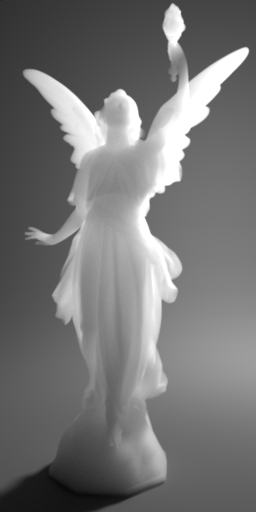
\includegraphics[height=\resLen]{images/lucy/N1_300nm.jpg} &
		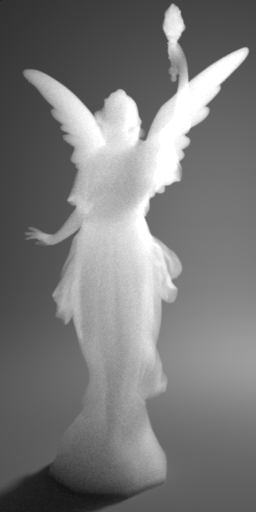
\includegraphics[height=\resLen]{images/lucy/N50_300nm.jpg} &
		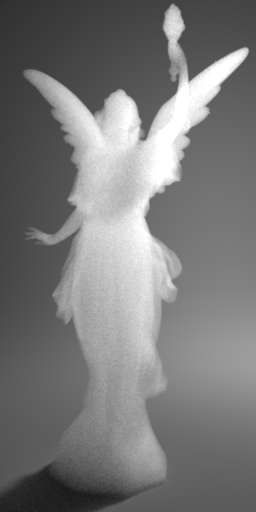
\includegraphics[height=\resLen]{images/lucy/N100_300nm.jpg} &
		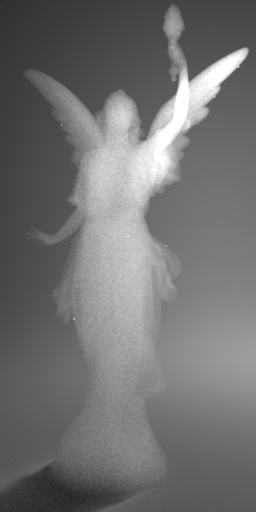
\includegraphics[height=\resLen]{images/lucy/N500_300nm.jpg}
		\\
		\raisebox{\raiseLen}{\rotatebox[origin=c]{90}{$\radius_i=400\text{nm}$}} &
		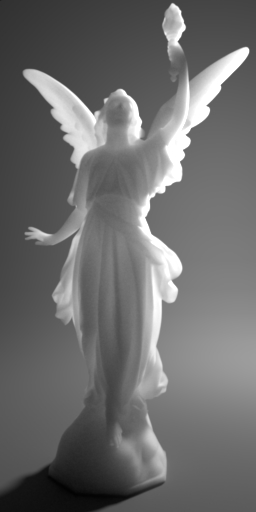
\includegraphics[height=\resLen]{images/lucy/N1_400nm.jpg} &
		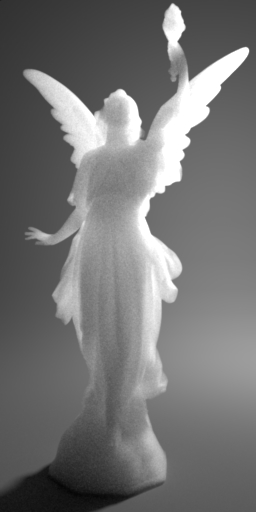
\includegraphics[height=\resLen]{images/lucy/N50_400nm.jpg} &
		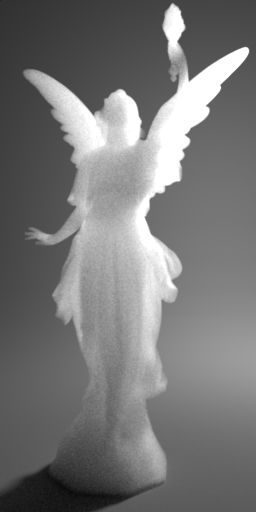
\includegraphics[height=\resLen]{images/lucy/N100_400nm.jpg} &
		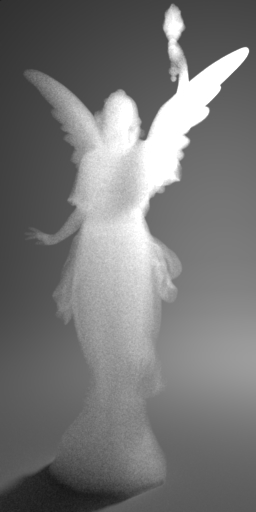
\includegraphics[height=\resLen]{images/lucy/N500_400nm.jpg}
		\\
		\raisebox{\raiseLen}{\rotatebox[origin=c]{90}{$\radius_i=500\text{nm}$}} &
		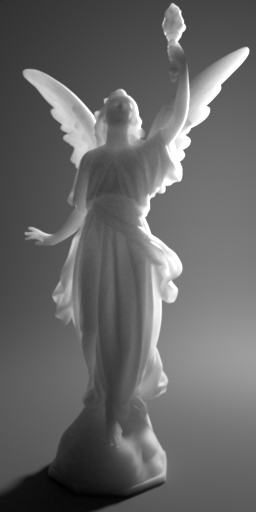
\includegraphics[height=\resLen]{images/lucy/N1_500nm.jpg} &
		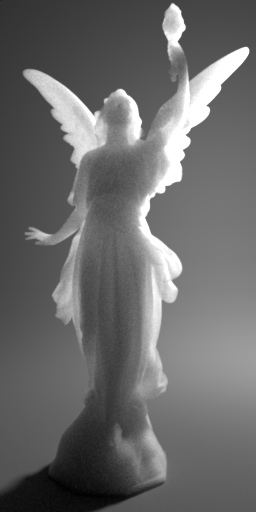
\includegraphics[height=\resLen]{images/lucy/N50_500nm.jpg} &
		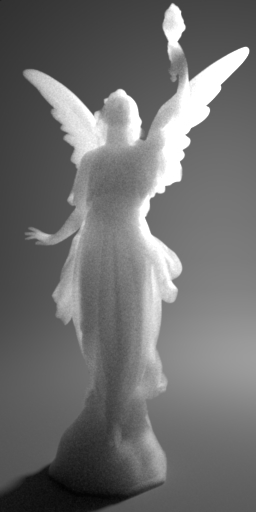
\includegraphics[height=\resLen]{images/lucy/N100_500nm.jpg} &
		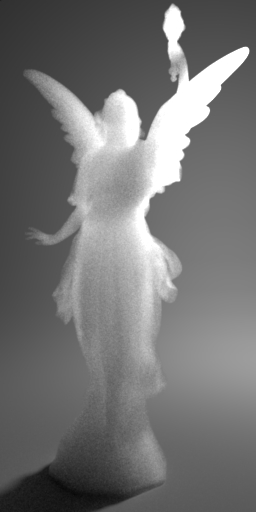
\includegraphics[height=\resLen]{images/lucy/N500_500nm.jpg}
	\end{tabular}
    \caption{\label{fig:lucycompare}
        Renderings of homogeneous Lucy models at $\lambda = 700\text{nm}$.
        The bulk scattering parameters are computed using our method with different combinations of particle radius~$\radius_i$ and per-cluster particle count~$\Ncls$.
    }
\end{figure}
